\documentclass{ximera}

\graphicspath{  
{./}
{./whoAreYou/}
{./drawingWithTheTurtle/}
{./bisectionMethod/}
{./circles/}
{./anglesAndRightTriangles/}
{./lawOfSines/}
{./lawOfCosines/}
{./plotter/}
{./staircases/}
{./pitch/}
{./qualityControl/}
{./symmetry/}
{./nGonBlock/}
}


%% page layout
\usepackage[cm,headings]{fullpage}
\raggedright
\setlength\headheight{13.6pt}


%% fonts
\usepackage{euler}

\usepackage{FiraMono}
\renewcommand\familydefault{\ttdefault} 
\usepackage[defaultmathsizes]{mathastext}
\usepackage[htt]{hyphenat}

\usepackage[T1]{fontenc}
\usepackage[scaled=1]{FiraSans}

%\usepackage{wedn}
\usepackage{pbsi} %% Answer font


\usepackage{cancel} %% strike through in pitch/pitch.tex


%% \usepackage{ulem} %% 
%% \renewcommand{\ULthickness}{2pt}% changes underline thickness

\tikzset{>=stealth}

\usepackage{adjustbox}

\setcounter{titlenumber}{-1}

%% journal style
\makeatletter
\newcommand\journalstyle{%
  \def\activitystyle{activity-chapter}
  \def\maketitle{%
    \addtocounter{titlenumber}{1}%
                {\flushleft\small\sffamily\bfseries\@pretitle\par\vspace{-1.5em}}%
                {\flushleft\LARGE\sffamily\bfseries\thetitlenumber\hspace{1em}\@title \par }%
                {\vskip .6em\noindent\textit\theabstract\setcounter{question}{0}\setcounter{sectiontitlenumber}{0}}%
                    \par\vspace{2em}
                    \phantomsection\addcontentsline{toc}{section}{\thetitlenumber\hspace{1em}\textbf{\@title}}%
                     }}
\makeatother



%% thm like environments
\let\question\relax
\let\endquestion\relax

\newtheoremstyle{QuestionStyle}{\topsep}{\topsep}%%% space between body and thm
		{}                      %%% Thm body font
		{}                              %%% Indent amount (empty = no indent)
		{\bfseries}            %%% Thm head font
		{)}                              %%% Punctuation after thm head
		{ }                           %%% Space after thm head
		{\thmnumber{#2}\thmnote{ \bfseries(#3)}}%%% Thm head spec
\theoremstyle{QuestionStyle}
\newtheorem{question}{}



\let\freeResponse\relax
\let\endfreeResponse\relax

%% \newtheoremstyle{ResponseStyle}{\topsep}{\topsep}%%% space between body and thm
%% 		{\wedn\bfseries}                      %%% Thm body font
%% 		{}                              %%% Indent amount (empty = no indent)
%% 		{\wedn\bfseries}            %%% Thm head font
%% 		{}                              %%% Punctuation after thm head
%% 		{3ex}                           %%% Space after thm head
%% 		{\underline{\underline{\thmname{#1}}}}%%% Thm head spec
%% \theoremstyle{ResponseStyle}

\usepackage[tikz]{mdframed}
\mdfdefinestyle{ResponseStyle}{leftmargin=1cm,linecolor=black,roundcorner=5pt,
, font=\bsifamily,}%font=\wedn\bfseries\upshape,}


\ifhandout
\NewEnviron{freeResponse}{}
\else
%\newtheorem{freeResponse}{Response:}
\newenvironment{freeResponse}{\begin{mdframed}[style=ResponseStyle]}{\end{mdframed}}
\fi



%% attempting to automate outcomes.

%% \newwrite\outcomefile
%%   \immediate\openout\outcomefile=\jobname.oc
%% \renewcommand{\outcome}[1]{\edef\theoutcomes{\theoutcomes #1~}%
%% \immediate\write\outcomefile{\unexpanded{\outcome}{#1}}}

%% \newcommand{\outcomelist}{\begin{itemize}\theoutcomes\end{itemize}}

%% \NewEnviron{listOutcomes}{\small\sffamily
%% After answering the following questions, students should be able to:
%% \begin{itemize}
%% \BODY
%% \end{itemize}
%% }
\usepackage[tikz]{mdframed}
\mdfdefinestyle{OutcomeStyle}{leftmargin=2cm,rightmargin=2cm,linecolor=black,roundcorner=5pt,
, font=\small\sffamily,}%font=\wedn\bfseries\upshape,}
\newenvironment{listOutcomes}{\begin{mdframed}[style=OutcomeStyle]After answering the following questions, students should be able to:\begin{itemize}}{\end{itemize}\end{mdframed}}



%% my commands

\newcommand{\snap}{{\bfseries\itshape\textsf{Snap!}}}
\newcommand{\flavor}{\link[\snap]{https://snap.berkeley.edu/}}
\newcommand{\mooculus}{\textsf{\textbf{MOOC}\textnormal{\textsf{ULUS}}}}


\usepackage{tkz-euclide}
\tikzstyle geometryDiagrams=[rounded corners=.5pt,ultra thick,color=black]
\colorlet{penColor}{black} % Color of a curve in a plot



\ifhandout\newcommand{\mynewpage}{\newpage}\else\newcommand{\mynewpage}{}\fi


\usepackage{multicol}


\author{Bart Snapp}

\checkYourselfAbstract

\begin{document}
\maketitle


%% begin{exercise}
%%   True or False: Concrete is measured in units of area.
%% \end{exercise}
%% \vfill

\begin{exercise}
  True or False: The dimensions of $3$ foot $2\times 4$ are $36\times
  2\times 4$ inches.
\end{exercise}
\vfill

\begin{exercise}
  True or False: $3$ square feet is equal to $36$ square inches.
 \end{exercise}
\vfill

\begin{exercise}
  You've been hired by the LEGO corporation to make a concrete statue
  of a LEGO minifigure:
  \begin{center}
    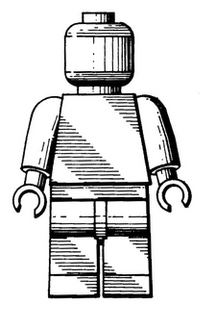
\includegraphics[width=1.5cm]{minifigure.png}
  \end{center}
  If the minifigure statue is around $7$' tall, around $3$' wide, and
  around $2$' deep, what's the most reasonable estimate for how many
  cubic yards of concrete are needed for the statue?
  \begin{enumerate}\begin{multicols}{2}
  \item around $2$ cubic yards
  \item around $4$ cubic yards
  \item around $16$ cubic yards
  \item around $32$ cubic yards
    \end{multicols}
  \end{enumerate}
\end{exercise}



\begin{exercise}
Stella and Tireale have identical LEGO minifigures. LEGO minifigures
are around $3.5$ centimeters tall, $1.5$ centimeters wide, and $1$
centimeter deep. Stella and Tireale both correctly measure their LEGO
minifigures.
\begin{multicols}{2}
  \begin{itemize}
\item Stella uses meters as units.
\item Tireale uses millimeters as units.
  \end{itemize}
\end{multicols}
Stella and Tireale both correctly compute the volume (V) and surface
area (SA) of their LEGO figures.  Which of the following could be
true? (SELECT ALL CORRECT ANSWERS)
\begin{multicols}{2}
\begin{enumerate}
\item Stella finds $SA > V$
\item Stella finds $SA < V$
\item Tireale finds $SA > V$
\item Tireale finds $SA < V$
\end{enumerate}
\end{multicols}
\end{exercise}



\begin{exercise}
  The MOOCulus Pizza Shop sells mini-pizzas that are $2$ inches in
  diameter. Assuming that the pizza shop uses the same crust for all
  of their pizzas, $9$ of these mini-pizzas is the same amount of food
  as\dots
  \begin{enumerate}
    \begin{multicols}{2}
    \item a pizza $6$'' in diameter
    \item a pizza $10$'' in diameter
    \item a pizza $14$'' in diameter
    \item a pizza $18$'' in diameter
    \end{multicols}
  \end{enumerate}
\end{exercise}




\answerlistbox{False}{False}{(a)}{(a) and (d)}{(a)}
\end{document}
